\documentclass{report}

\usepackage{hyperref}
\usepackage{graphicx}
\usepackage{booktabs}
\graphicspath{{./imgs}}

\begin{document}
    
    \chapter*{Introduzione}
        Il progetto consiste nella comparazione delle prestazioni di alcuni ambienti di sviluppo per quanto riguarda
        la fattorizzazione di Cholesky di matrici sparse.\\
        L'obiettivo è quello di individuare l'ambiente di sviluppo open source che presenta le migliori prestazioni
        in termini di tempo di esecuzione, memoria utilizzata e precisione della soluzione.\\

    \chapter[Enviroments]{Ambienti di sviluppo}
        Sono qui riportati i dettagli riguardo gli ambienti di sviluppo utilizzati, 
        dividendo per linguaggio di programmazione la descrizione delle librerie utilizzate.

        \section{MATLAB}
            MATLAB supporta nativamente le matrici sparse e la fattorizzazione di Cholesky.
            Il metodo \texttt{chol} è stato utilizzato per calcolare la fattorizzazione e
            l'operatore \verb$\$ per risolvere il sistema lineare.

        \section{Java}
            La libreria Java EJML è stata utilizzata per la rappresentazione sparsa delle matrici
            e per la fattorizzazione di Cholesky.
            I file \texttt{.mat} sono stati caricati con l'aiuto della libreria MFL.
            Risulta importante notare la presenza di alcune limitazioni nella libreria EJML,
            tra le quali la più importante è l'impossibilità di applicare la fattorizzazione di Cholesky
            su matrici di grandi dimensioni a causa dell'utilizzo di interi a per l'indicizzazione degli array.
            Questa limitazione è nota agli sviluppatori ma al momento della stesura di questo documento rimane
            una problematica non risolta.

            \begin{itemize}
                \item \href{http://ejml.org/}{EJML}
                \item \href{https://github.com/HebiRobotics/MFL}{MFL}
            \end{itemize}
            
        \section{Python}
            La libreria SciPy è stata utilizzata per per le matrici sparese insieme a scikit-sparse per la 
            fattorizzazione di Cholesky.
            SciPy offre inoltre le funzionalità per la lettura dei file \texttt{.mat}.
            La fattorizzazione di Cholesky è implementata dal modulo sksparse.cholmod, che a sua volta si basa sulla
            libreria open source cholmod, scritta in C e parte di SuiteSparse.
            \`E da segnalare la mancaza del modulo sksparse.cholmod, necessario per la fattorizzazione, tramite il 
            packet manager \texttt{pip} sui sistemi Windows, il modulo è stato compilato e installato seguendo le
            istruzioni presenti sul 
            \href{https://github.com/xmlyqing00/Cholmod-Scikit-Sparse-Windows}{repository github di xmlqing00}.

            \begin{itemize}
                \item \href{https://www.scipy.org/}{SciPy}
                \item \href{https://github.com/scikit-sparse/scikit-sparse} {scikit-sparse}
                \item \href{http://suitesparse.com}{SuiteSparse}
            \end{itemize}

        \section{Julia}
            Il package SparseArrays mette a disposizione le classi per le matrici sparse, mentre la fattorizzazione di 
            Cholesky
            è implementata dal package LinearAlgebra.
            Il package MAT è stato utilizzato per la lettura dei file \texttt{.mat}.
            L'implementazione della fattorizzazione di Cholesky del package LinearAlgebra si basa sulla libreria cholmod
            della suite di librerie SuiteSparse.

            \begin{itemize}
                \item \href{https://docs.julialang.org/en/v1/stdlib/SparseArrays/}{SparseArrays}
                \item \href{https://docs.julialang.org/en/v1/stdlib/LinearAlgebra/}{LinearAlgebra}
                \item \href{https://github.com/JuliaIO/MAT.jl}{MAT}
                \item \href{http://suitesparse.com}{SuiteSparse}
            \end{itemize}

    \chapter{Benchmarks}
        I benchmark sono stati eseguiti una volta per ogni ambiente di sviluppo e per ogni matrice, sia in un sistema
        Windows che in un sistema Linux, utilizzando la stessa macchina.
        In particolare è stato utilizzato un processore ad 8 core AMD Ryzen 7 PRO 6850U a 2.70 GHz con 32 GB di RAM.

        \section{Modalità di misurazione}

            Le misurazioni sono effettuate sulla risoluzione del sistema $Ax = b$ dove il termine noto $b$ è calcolato
            in modo tale che $b = A*xe$ con $xe$ vettore di tutti 1.\\

            \begin{itemize}
                \item \textbf{TIME}: il tempo di computazione è calcolato dal momento in cui la matrice è completamente
                caricata in memoria nel corretto formato per l'esecuzione della fattorizzazione di Cholesky fino al 
                momento in cui il sistema lineare è risolto. In generale il tempo di computazione comprende anche il 
                tempo in cui il processo è in stato ready ma non è in esecuzione su nessun core.
                \item \textbf{MEMORY USAGE}: la memoria utilizzata è stimata come la differenza tra la memoria occupata 
                dal processo prima dell'esecuzione e quella occupata dal processo subito dopo la risoluzione.
                A causa della natura degli ambienti utilizzati la misurazione della memoria può essere difficile e 
                risultare particolarmente inaccurata. In particolare Java, essendo eseguito in una virtual machine e
                utilizzando un garbage collector potrebbe produrre risultati poco affidabili.\\
                Inoltre, a seconda dell'ambiente, l'implementazione delle funzioni native per il profiling potrebbe 
                variare e misurare in modo diverso la memoria, in particolare tra sistemi operativi diversi anche lo 
                stesso linguaggio potrebbe presentare implementazioni differenti.
                \item \textbf{RELATIVE ERROR}: l'errore relativo è calcolato come $||x-xe||/||xe||$, ovvero la norma 
                della differenza tra la soluzione ottentuta con la decomposizione di Cholesky e il vettore di 
                riferimento tutti 1. Il vettore dei temini noti $b$ è calcolato come $b = A*xe$ da ciascun ambiente.
                Per quanto i vettori così calcolati siano in generale affidabili, potrebbero presentare delle differenze
                tra i diversi ambienti per quanto riguarda la precisione della soluzione. Un approccio più preciso 
                sarebbe stato quello di utilizzare lo stesso vettore precalcolato per tutti gli ambienti.
            \end{itemize}

        \section{Matrici}
            Sono state utilizzate per i benchmark nove matrici sparese messe a disposizione sul sito web 
            \href{https://sparse.tamu.edu/}{The SuiteSparse Matrix Collection}. Le matrici sono di diverse dimensioni 
            e densità. In particolare in Table~\ref{tab:matrices} sono riportati i dettagli delle matrici utilizzate.

            \begin{table}[h]
                \centering
                
                \begin{tabular}{@{}lrrr@{}}
                \toprule
                \textbf{Nome}   
                & \textbf{Dimensione} & \textbf{Nonzero} & \textbf{Densità} \\ 
                \midrule
                \href{https://sparse.tamu.edu/FIDAP/ex15}{ex15}            
                & 6\,867         & 98\,671          & 0.2092\%         \\
                \href{https://sparse.tamu.edu/MaxPlanck/shallow_water1}{shallow\_water1} 
                & 81\,920        & 327\,680         & 0.0049\%         \\ 
                \href{https://sparse.tamu.edu/Rothberg/cfd1}{cfd1}            
                & 70\,656        & 1\,825\,580      & 0.0366\%         \\
                \href{https://sparse.tamu.edu/Rothberg/cfd2}{cfd2}            
                & 123\,440       & 3\,085\,406      & 0.0202\%         \\
                \href{https://sparse.tamu.edu/Wissgott/parabolic_fem}{parabolic\_fem}  
                & 525\,825       & 3\,674\,625      & 0.0013\%         \\
                \href{https://sparse.tamu.edu/GHS_psdef/apache2}{apache2}         
                & 715\,176       & 4\,817\,870      & 0.0009\%         \\
                \href{https://sparse.tamu.edu/AMD/G3_circuit}{G3\_circuit}     
                & 1\,585\,478    & 7\,660\,826      & 0.0003\%         \\
                \href{https://sparse.tamu.edu/Janna/StocF-1465}{StocF-1465}      
                & 1\,465\,137    & 21\,005\,389     & 0.0010\%         \\
                \href{https://sparse.tamu.edu/Janna/Flan_1565}{Flan\_1565}      
                & 1\,564\,794    & 114\,165\,372    & 0.0047\%         \\
                \bottomrule
                \end{tabular}%
                
                \caption{Sommario delle matrici utilizzate nei benchmark.}
                \label{tab:matrices}
                \end{table}
        
        \section{Results}
            In questa sezione sono riportati i risultati dei benchmark suddivisi per ambiente di sviluppo.
            \subsection{MATLAB}
                Nella Table~\ref{tab:result_matlab} sono riportati i risultati ottenuti utilizzando MATLAB.
                Si può osservare come i tempi di esecuzione e la memoria utilizzata crescano al crescere del numeri di
                elementi non nulli della matrice.\\
                Osservando i risultati dell'utilizzo della memoria si può notare come per la matrice \texttt{cfd2.mat}
                in ambiente Linux sia stata utilizzata una quantità di memoria molto elevata. Si presume che questo
                sia un errore dovuto al calolo della memoria dell'ambiente MATLAB.\\
                In Figure~\ref{fig:matlab_overflow} è riportato il comando MATLAB utilizzato per il calcolo della 
                memoria utilizzata ed è possibile vedere come il valore restituito per la matrice \texttt{cfd2.mat} sia
                molto elevato mentre quello restituito per la matrice \texttt{cfd1.mat} sia molto più contenuto.
                \begin{figure}[h]
                    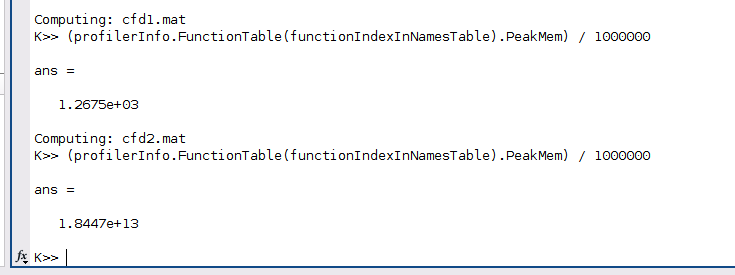
\includegraphics[width=\textwidth]{matlab_overflow}
                    \caption{Comando MATLAB utilizzato per la profilazione della memoria}
                    \label{fig:matlab_overflow}
                \end{figure}\\
                \`E interessante notare come MATLAB utilizzando la funzione \texttt{chol} non riesca a fattorizzare
                tutte le matrici testate perché termina la memoria a disposizione mentre utilizzando direttamente
                l'operatore \verb$\$ non presenta questo problema.\\
                \begin{table}[h]
                    \centering
                    \resizebox{\columnwidth}{!}{%
                    \begin{tabular}{@{}lrrrrrcc@{}}
                    \toprule
                    \textbf{A} &
                    \textbf{size} &
                    \textbf{NNZ} &
                    \textbf{time {[}s{]}} &
                    \textbf{memory\_usage {[}MB{]}} &
                    \textbf{relative\_error} &
                    \textbf{platform} &
                    \textbf{library\_version} \\ \midrule
                    ex15.mat            & 6867   & 98671   & 0.05   & 4.19              & 8.21380E-07 & LINUX   & 9.14.0.2254940 (R2023a) Update 2 \\
                    ex15.mat            & 6867   & 98671   & 0.06   & 4.15              & 8.21380E-07 & WINDOWS & 9.13.0.2193358 (R2022b) Update 5 \\
                    shallow\_water1.mat & 81920  & 327680  & 1.72   & 368.87            & 3.07689E-16 & LINUX   & 9.14.0.2254940 (R2023a) Update 2 \\
                    shallow\_water1.mat & 81920  & 327680  & 2.09   & 368.93            & 3.07689E-16 & WINDOWS & 9.13.0.2193358 (R2022b) Update 5 \\
                    cfd1.mat            & 70656  & 1825580 & 3.86   & 1286.22           & 6.34538E-13 & LINUX   & 9.14.0.2254940 (R2023a) Update 2 \\
                    cfd1.mat            & 70656  & 1825580 & 6.54   & 1302.86           & 6.34538E-13 & WINDOWS & 9.13.0.2193358 (R2022b) Update 5 \\
                    cfd2.mat            & 123440 & 3085406 & 6.55   & 18446744071912.70 & 7.98365E-13 & LINUX   & 9.14.0.2254940 (R2023a) Update 2 \\
                    cfd2.mat            & 123440 & 3085406 & 13.07  & 2503.08           & 7.98365E-13 & WINDOWS & 9.13.0.2193358 (R2022b) Update 5 \\
                    apache2.mat         & 715176 & 4817870 & 646.19 & 27490.58          & 3.65750E-11 & WINDOWS & 9.13.0.2193358 (R2022b) Update 5 \\ \bottomrule
                    \end{tabular}%
                    }
                    \caption{Risultati dei benchmark MATLAB}
                    \label{tab:result_matlab}
                \end{table}
            \subsection{Java}
                Osservando i risultati nella Table~\ref{tab:result_java} si può notare come l'errore relativo e la 
                memoria utilizzata per ogni matrice sia stabile tra i due sistemi operativi, mentre il tempo di 
                computazione è più variabile pur non discostandosi molto.\\
                Le matrici fattorizzate nei due sistemi operativi sono le stesse in quanto i limiti non derivano tanto
                dal memoria disponibile quanto dai limiti della libreria utilizzata. Infatti la libreria EJML utilizza
                interi a 32 bit con segno per indicizzare gli elementi della matrice e nella fattorizzazione di Cholesky
                non è in grado di gestire matrici con più di $2^{31}$ elementi.
                \begin{table}[h]
                    \centering
                    \resizebox{\columnwidth}{!}{%
                    \begin{tabular}{@{}lrrrrrcc@{}}
                    \toprule
                    \textbf{A} &
                    \textbf{size} &
                    \textbf{NNZ} &
                    \textbf{time {[}s{]}} &
                    \textbf{memory\_usage {[}MB{]}} &
                    \textbf{relative\_error} &
                    \textbf{platform} &
                    \textbf{library\_version} \\ \midrule
                    ex15.mat            & 6867   & 98671   & 0.01   & 5.12    & 8.00799E-07 & LINUX   & 0.43 \\
                    ex15.mat            & 6867   & 98671   & 0.01   & 5.01    & 8.00799E-07 & WINDOWS & 0.43 \\
                    shallow\_water1.mat & 81920  & 327680  & 10.42  & 290.06  & 3.55914E-16 & LINUX   & 0.43 \\
                    shallow\_water1.mat & 81920  & 327680  & 8.96   & 291.21  & 3.55914E-16 & WINDOWS & 0.43 \\
                    cfd1.mat            & 70656  & 1825580 & 76.96  & 992.04  & 4.52430E-11 & LINUX   & 0.43 \\
                    cfd1.mat            & 70656  & 1825580 & 119.12 & 991.02  & 4.52430E-11 & WINDOWS & 0.43 \\
                    cfd2.mat            & 123440 & 3085406 & 121.92 & 1927.05 & 2.19321E-11 & LINUX   & 0.43 \\
                    cfd2.mat            & 123440 & 3085406 & 121.14 & 1928.13 & 2.19321E-11 & WINDOWS & 0.43 \\ \bottomrule
                    \end{tabular}%
                    }
                    \caption{Risultati dei benchmark Java}
                    \label{tab:result_java}
                \end{table}
            \subsection{Python}
                Come mostrano i risultati nella Table~\ref{tab:result_python} l'implementazione Windows risulta essere 
                generalmente meno precisa rispetto all'implementazione Linux. 
                I tempi di calcolo oscillano a favore dell'uno o dell'altro sistema operativo a seconda della matrice
                con differenze anche significative che non permettono però di identificare un sistema come più
                veloce dell'altro.
                L'utilizzo della memoria utilizzando un sistema Windows risulta essere più contenuto, ma il sistema
                linux ha permesso di fattorizzare anche le matrici più grandi, dove invece Windows termina la memoria.
                \begin{table}[h]
                    \centering
                    \resizebox{\columnwidth}{!}{%
                    \begin{tabular}{@{}lrrrrrcc@{}}
                    \toprule
                    \textbf{A} &
                    \textbf{size} &
                    \textbf{NNZ} &
                    \textbf{time {[}s{]}} &
                    \textbf{memory\_usage {[}MB{]}} &
                    \textbf{relative\_error} &
                    \textbf{platform} &
                    \textbf{library\_version} \\ \midrule
                    ex15.mat            & 6867    & 98671     & 0.94   & 726.99  & 3.49945E-07 & LINUX   & 1.8.1  \\
                    ex15.mat            & 6867    & 98671     & 0.02   & 78.57   & 3.97177E-07 & WINDOWS & 1.10.1 \\
                    shallow\_water1.mat & 81920   & 327680    & 4.00   & 726.99  & 3.27712E-16 & LINUX   & 1.8.1  \\
                    shallow\_water1.mat & 81920   & 327680    & 0.69   & 84.01   & 3.75545E-16 & WINDOWS & 1.10.1 \\
                    cfd1.mat            & 70656   & 1825580   & 3.62   & 499.01  & 1.11282E-11 & LINUX   & 1.8.1  \\
                    cfd1.mat            & 70656   & 1825580   & 45.51  & 105.17  & 2.47670E-11 & WINDOWS & 1.10.1 \\
                    cfd2.mat            & 123440  & 3085406   & 8.65   & 499.15  & 1.65638E-11 & LINUX   & 1.8.1  \\
                    cfd2.mat            & 123440  & 3085406   & 130.17 & 121.55  & 3.41646E-11 & WINDOWS & 1.10.1 \\
                    parabolic\_fem.mat  & 525825  & 3674625   & 19.52  & 726.99  & 1.91515E-11 & LINUX   & 1.8.1  \\
                    parabolic\_fem.mat  & 525825  & 3674625   & 22.07  & 144.30  & 2.35390E-11 & WINDOWS & 1.10.1 \\
                    apache2.mat         & 715176  & 4817870   & 82.83  & 551.96  & 1.70028E-10 & LINUX   & 1.8.1  \\
                    apache2.mat         & 715176  & 4817870   & 270.27 & 171.90  & 2.24076E-10 & WINDOWS & 1.10.1 \\
                    G3\_circuit.mat     & 1585478 & 7660826   & 87.47  & 785.36  & 3.34037E-11 & LINUX   & 1.8.1  \\
                    G3\_circuit.mat     & 1585478 & 7660826   & 328.09 & 244.55  & 5.82245E-11 & WINDOWS & 1.10.1 \\
                    StocF-1465.mat      & 1465137 & 21005389  & 376.75 & 739.66  & 1.89743E-08 & LINUX   & 1.8.1  \\
                    Flan\_1565.mat      & 1564794 & 114165372 & 447.43 & 1893.95 & 5.33502E-10 & LINUX   & 1.8.1  \\ \bottomrule
                    \end{tabular}%
                    }
                    \caption{Risultati dei benchmark Python}
                    \label{tab:result_python}
                \end{table}
            
                \subsection{Julia}
                La Table~\ref{tab:result_julia} riporta i risultati ottenuti utilizzando Julia. Si può notare come
                l'utilizzo della memoria è sempre stabile tra i due sistemi operativi così come l'errore 
                relativo si discosta di valori poco significativi, ma i tempi di calcolo sono spesso favorevoli in 
                ambiente Windows. In ambiente Windows è stato inoltre possibile fattorizzare tutte le matrici.
                \begin{table}[h]
                    \centering
                    \resizebox{\columnwidth}{!}{%
                    \begin{tabular}{@{}lrrrrrcc@{}}
                    \toprule
                    \textbf{A} &
                    \textbf{size} &
                    \textbf{NNZ} &
                    \textbf{time {[}s{]}} &
                    \textbf{memory\_usage {[}MB{]}} &
                    \textbf{relative\_error} &
                    \textbf{platform} &
                    \textbf{library\_version} \\ \midrule
                    ex15.mat            & 6867    & 98671     & 0.03   & 11.48    & 5.81497E-07 & LINUX   & 1.9.0 \\
                    ex15.mat            & 6867    & 98671     & 0.02   & 11.48    & 5.81497E-07 & WINDOWS & 1.9.0 \\
                    shallow\_water1.mat & 81920   & 327680    & 0.55   & 75.02    & 2.01653E-16 & LINUX   & 1.9.0 \\
                    shallow\_water1.mat & 81920   & 327680    & 0.15   & 75.02    & 2.01653E-16 & WINDOWS & 1.9.0 \\
                    cfd1.mat            & 70656   & 1825580   & 1.49   & 540.85   & 7.06626E-14 & LINUX   & 1.9.0 \\
                    cfd1.mat            & 70656   & 1825580   & 1.59   & 540.36   & 6.17525E-14 & WINDOWS & 1.9.0 \\
                    cfd2.mat            & 123440  & 3085406   & 2.66   & 1019.36  & 3.07576E-13 & LINUX   & 1.9.0 \\
                    cfd2.mat            & 123440  & 3085406   & 2.34   & 1019.36  & 2.74264E-13 & WINDOWS & 1.9.0 \\
                    parabolic\_fem.mat  & 525825  & 3674625   & 3.40   & 771.37   & 7.12844E-13 & LINUX   & 1.9.0 \\
                    parabolic\_fem.mat  & 525825  & 3674625   & 2.05   & 771.37   & 7.10019E-13 & WINDOWS & 1.9.0 \\
                    apache2.mat         & 715176  & 4817870   & 7.99   & 2346.68  & 5.60339E-11 & LINUX   & 1.9.0 \\
                    apache2.mat         & 715176  & 4817870   & 6.52   & 2346.68  & 5.60359E-11 & WINDOWS & 1.9.0 \\
                    G3\_circuit.mat     & 1585478 & 7660826   & 12.46  & 3070.81  & 4.88705E-12 & LINUX   & 1.9.0 \\
                    G3\_circuit.mat     & 1585478 & 7660826   & 8.60   & 3070.81  & 4.88457E-12 & WINDOWS & 1.9.0 \\
                    StocF-1465.mat      & 1465137 & 21005389  & 483.85 & 39483.77 & 2.38859E-10 & WINDOWS & 1.9.0 \\
                    Flan\_1565.mat      & 1564794 & 114165372 & 538.93 & 43646.98 & 1.67777E-12 & WINDOWS & 1.9.0 \\ \bottomrule
                    \end{tabular}%
                    }
                    \caption{Risultati dei benchmark Julia}
                    \label{tab:result_julia}
                \end{table}
            
        \section{Comparazione}

    \chapter{Conclusioni}
        Anzitutto è evidente come gli unici ambienti in cui è stato possibile fattorizzare tutte le matrici sono 
        stati Python e Julia, in particolare solo in sistema Linux per Python e in Windows per Julia. 
        \`E interessante notare che la libreria Python non ha raggiunto gli stessi risultati in fatto di precisione
        dei risultati nonostante utilizzi per la fattorizzazione la stessa libreria.\\
        Julia risulta essere l'ambiente dove l'errore relativo registrato è minore nella maggior parte 
        dei casi. 
        Per quanto riguarda i tempi di computazione Julia risulta essere l'ambiente più veloce in quasi ogni caso.\\
        In generale si può notare come il caso in cui Julia ottiene risultati peggiori rispetto agli altri è quello 
        con la matrice ex15, ovvero la più piccola delle matrici ma anche la più densa, questo potrebbe suggerire 
        che la libreria perda in prestazioni all'aumentare della densità più delle altre, ma maggiori test sarebbero
        necessari per confermare questa ipotesi.\\
        In ambiente Python sono registrati le minori variazioni nella memoria occupata con la maggior parte delle
        matrici testate trovando ancora una volta nella matrice ex15 l'eccezione.\\
        In conclusione Julia sembrerebbe essere l'ambiente più performante sia in termini di tempo di esecuzione che
        di precisione della soluzione e pur non essendo il meglio ottimizzato nell'utilizzo della memoria risulta
        essere l'unico ambiente in cui è stato possibile fattorizzare tutte le matrici testate.

            
                
\end{document}
